\section{Trabalhos Correlatos}

Nos últimos anos, a aplicação de \acp{mllm} na análise de imagens médicas se tornou mais comum. Em uma revisão
sistemática de \textcite{eric2025systematic}, é avaliado o estado da arte, contemplando os principais avanços e
desafios nesta área. Em geral, a maioria dos \acp{mllm} que possuem alguma capacidade de análise de imagens
dermatológicas são generalistas e não apresentam uma avaliação aprofundada de suas capacidades de classificação ou
descrição de lesões de pele. Porém, há modelos especializados para a dermatologia, como o SkinGPT-4 de
\textcite{zhou2023skingpt}. Nas subseções abaixo, serão apresentados alguns modelos que possuem aplicações na
dermatologia.

\subsection{SkinGPT-4}

O modelo SkinGPT-4 foi proposto e desenvolvido por \textcite{zhou2023skingpt} e se baseia no Mini\ac{gpt}-4, um
\ac{mllm} composto por um \ac{vit} com um \textit{Q-Former} pré-treinado e o \ac{llm} Vicuna, que por sua vez é baseado
no \ac{llama}. Este \ac{mllm} foi desenvolvido para tarefas de pergunta e resposta visuais, também conhecidas como
\ac{vqa}. A arquitetura pode ser vista na \autoref{fig:skingpt4}.

\clearpage

\begin{figure}[ht]
    \centering
    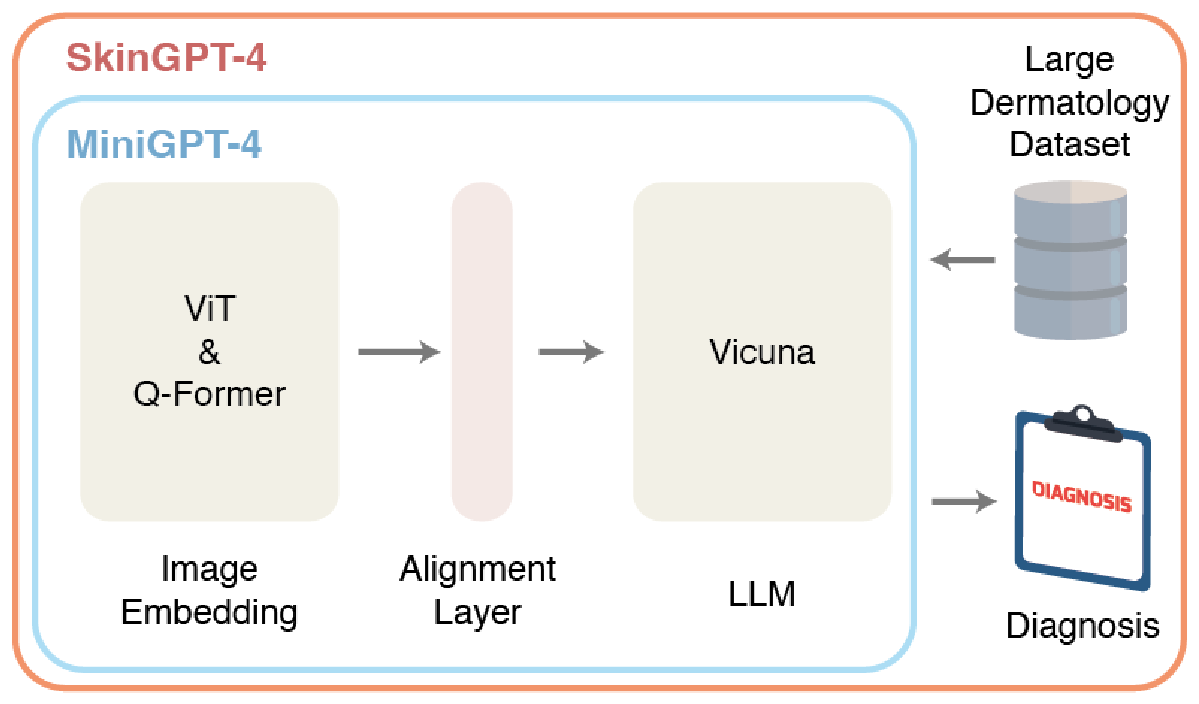
\includegraphics[width=0.55\columnwidth,keepaspectratio]{images/skingpt4.png}
    \label{fig:skingpt4}
    \caption{Arquitetura do Skin\ac{gpt}-4. Fonte: \textcite{zhou2023skingpt}.}
\end{figure}

Neste estudo, o Mini\ac{gpt}-4 passou por um processo de \textit{fine-tuning} de duas etapas que familiarizou o modelo
com imagens de lesões de pele e depois ajustou suas saídas para um formato mais próximo de um diagnóstico médico. As
imagens vieram de um conjunto de dados particular, do SKINCON e do Dermnet, sendo que 3886 imagens foram usadas na
primeira etapa de treinamento e 49043 na segunda.

A verificação do desempenho do modelo foi feito com base em 150 diagnósticos de casos reais realizados pelo
Skin\ac{gpt}-4. Esses diagnósticos foram avaliados por dermatologistas certificados, sendo que 78,76\% dos diagnósticos
foram classificados como corretos.

\subsection{MpoxVLM}

O modelo MpoxVLM de \textcite{cao2024mpoxvlm} é um \ac{mllm} direcionado ao diagnóstico de lesões de pele causadas pela
doença \textit{Monkeypox}. O modelo possui dois codificadores visuais, um deles é o \ac{clip} \ac{vit}-L/14 e o outro é
o \ac{vit}-L/14-336 pré-treinado para a classificação de lesões de pele. Um \ac{mlp} de duas camadas é usado como
projetor de entrada para o codificador \ac{clip}, sendo que a saída do codificador \ac{vit}, a classe da lesão de pele,
é enviada para outro projetor de entrada. O \ac{llama}-2 é usado como \ac{llm}, especificamente a variante com 7
bilhões de parâmetros. A \autoref{fig:mpoxvlm} apresenta a arquitetura deste \ac{mllm}.

\clearpage

\begin{figure}[ht]
    \centering
    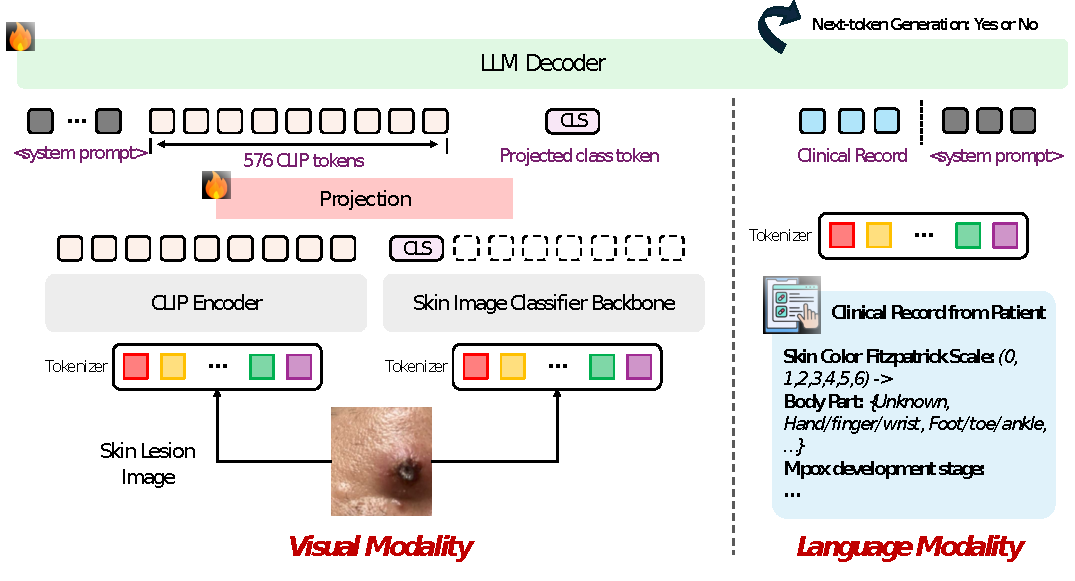
\includegraphics[width=0.85\columnwidth,keepaspectratio]{images/mpoxvlm.pdf}
    \label{fig:mpoxvlm}
    \caption{Arquitetura do MpoxVLM. Fonte: \textcite{cao2024mpoxvlm}.}
\end{figure}

Inicialmente, o \ac{vit}-L/14-336 foi pré-treinado com o conjunto de dados de lesões de pele causadas por
\textit{Monkeypox}. Depois o modelo foi construído e os projetores de entrada foram treinados. Por fim, foi feito um
\textit{fine-tuning} com \ac{lora} do \ac{llama}-2 para tarefas de \ac{vqa}. Foram utilizadas duas NVIDIA RTX 4090 para
os treinamentos neste estudo.

Os resultados apresentados demonstram que o MpoxVLM atinge uma acurácia de 90,38\% no diagnóstico de
\textit{Monkeypox}, ultrapassando vários outros \acp{mllm}.

\subsection{MedPLIB}

O MedPLIB de \textcite{huang2025towards} é um \ac{mllm} generalista que foca no entendimento de imagens a nível de
pixel, oferecendo suporte para vários formatos de \textit{prompt}, como os de \ac{vqa} e de descrição de regiões ou
pontos. O modelo utiliza o codificador visual \ac{clip} Large de \textcite{radford2021learning}, o \ac{llm}
\ac{llama}-2 com 7 bilhões de parâmetros e o modelo para segmentação de imagens \ac{sam-med2d} de
\textcite{cheng2023sam} como decodificador para o foco em áreas específicas da imagem.

A arquitetura do MedPLIB é organizada como uma \ac{moe}, dessa forma, múltiplos modelos são treinados com focos em
diferentes domínios, levando ao aumento do desempenho. O \textit{fine-tuning} foi realizado em quatro estágios,
começando com o alinhamento das respostas textuais e seguindo com o treinamento visual para o \ac{vqa}. Depois, o
decodificador utilizado na segmentação e identificação de regiões foi treinado e o processo foi finalizado com um
treinamento completo sobre todos os componentes do modelo. A \autoref{fig:medblib} apresenta a arquitetura do MedPLIB.

\clearpage

\begin{figure}[ht]
    \centering
    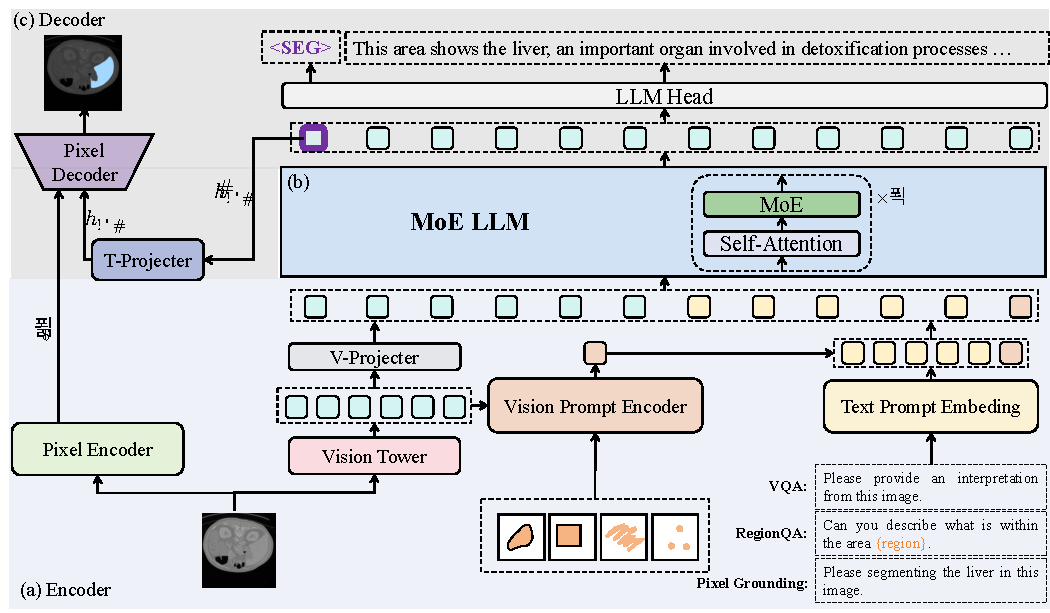
\includegraphics[width=0.8\columnwidth,keepaspectratio]{images/medblip.pdf}
    \label{fig:medblib}
    \caption{Arquitetura do MedBLIP. Fonte: \textcite{huang2025towards}.}
\end{figure}

O estudo apresenta avaliações na área da dermatologia com o \textit{benchmark} OmniMedVQA de
\textcite{hu2024omnimedvqa}, que avalia o desempenho em tarefas de \ac{vqa}. Os resultados podem ser conferidos na
\autoref{tab:medblip_dermatology_results}.

\begin{table}[ht]
    \centering
    \begin{tabular}{l|c}
        \hline
        Modelo                 & Pontuação      \\ \hline
        MiniGPT-4              & 41,28          \\
        BLIP-2                 & 40,93          \\
        InstructBLIP           & \textbf{63,02} \\
        \ac{llava}             & 49,67          \\
        VPGTrans               & 45,42          \\
        RadFM                  & 38,32          \\
        \ac{llava}-Med         & 46,42          \\
        LISA                   & 41,61          \\ \hline
        MedPLIB (sem \ac{moe}) & 43,37          \\
        MedPLIB                & 51,47          \\ \hline
    \end{tabular}
    \label{tab:medblip_dermatology_results}
    \caption{Comparação entre modelos no \textit{benchmark} OmniMedVQA em dermatologia. A pontuação máxima está
    destacada. Fonte: \textcite{hu2024omnimedvqa}.}
\end{table}

\subsection{UMed-LVLM}

O modelo UMed-LVLM, desenvolvido por \textcite{zhou2025training}, é generalista e foca em aprimorar a capacidade de
localização de anormalidades médicas em imagens. Este modelo baseia-se no MedVInt de \textcite{zhang2023pmc} e é
treinado em duas etapas, sendo que a primeira realiza um \textit{fine-tuning} com o método \textit{Abnormal-Aware
Instruction Tuning} e a segunda aplica \ac{ppo} com o método \textit{Abnormal-Aware Rewarding}.

\clearpage

\begin{figure}[ht]
    \centering
    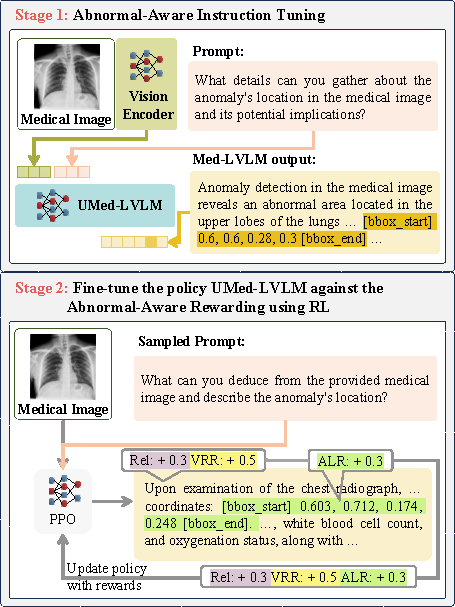
\includegraphics[width=0.5\columnwidth,keepaspectratio]{images/umedlvlm.pdf}
    \label{fig:umedlvlm}
    \caption{Processo de treinamento do UMed-LVLM. Fonte: \textcite{zhou2025training}.}
\end{figure}

O artigo apresenta a avaliação da acurácia em diagnósticos dermatológicos do UMed-LVLM. Os testes foram realizados
com o conjunto de dados MedMNIST de \textcite{yang2021medmnist}. A \autoref{tab:umedlvlm_acc} traz os resultados da
avaliação.

\begin{table}[ht]
    \centering
    \begin{tabular}{l|c}
        \hline
        Modelo        & Acurácia      \\ \hline
        ResNet50      & 73,1          \\
        DWT-CV        & 74,8          \\
        SADAE         & 75,9          \\
        PMC-\ac{clip} & 79,8          \\
        MedVInT       & 80,0          \\ \hline
        UMed-LVLM     & \textbf{84,1} \\ \hline
    \end{tabular}
    \label{tab:umedlvlm_acc}
    \caption{Comparação entre modelos com a seção de dermatologia do conjunto de dados MedMNIST. A pontuação
    máxima está destacada em negrito. Fonte: \textcite{zhou2025training}.}
\end{table}

\subsection{UMIT}

UMIT é um \ac{mllm} generalista desenvolvido por \textcite{yu2025umit} que tem como objetivo suportar \ac{vqa} em
várias áreas da medicina. O modelo foi treinado a partir do \ac{mllm} Qwen2-VL de \textcite{wang2024qwen2} e utilizou
um regime de duas etapas no seu treinamento. A primeira etapa alinhou as informações das imagens médicas com as
informações textuais. Na segunda etapa, o \textit{fine-tuning} do modelo foi realizado, adaptando-o para diversas
tarefas de \ac{vqa}. A \autoref{fig:umit} mostra a arquitetura e o processo de treinamento do modelo UMIT.

\begin{figure}[ht]
    \centering
    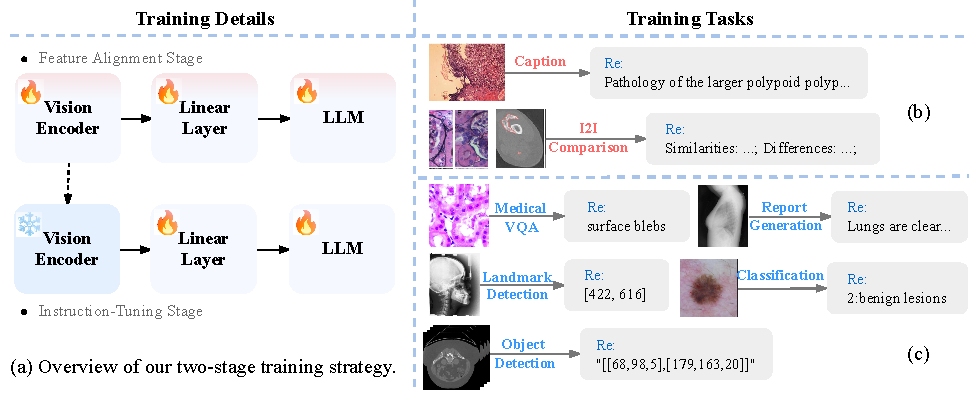
\includegraphics[width=0.8\columnwidth,keepaspectratio]{images/umit.pdf}
    \label{fig:umit}
    \caption{(a): Processo de treinamento e arquitetura do UMIT. (b) Primeira etapa de treinamento (c):
    Segunda etapa de treinamento. Fonte: \textcite{yu2025umit}.}
\end{figure}

A acurácia do modelo em diagnósticos foi avaliada com a seção de dermatologia do conjunto de dados MedMNIST e pode ser
conferida na \autoref{tab:umit_acc}.

\begin{table}[ht]
    \centering
    \begin{tabular}{l|c}
        \hline
        Modelo      & Acurácia       \\ \hline
        Qwen2-vl    & 11,3           \\
        BiomedGPT-S & 75,2           \\
        BiomedGPT-M & 78,0           \\
        BiomedGPT-B & 78,6           \\ \hline
        UMIT        & \textbf{82,54} \\ \hline
    \end{tabular}
    \label{tab:umit_acc}
    \caption{Comparação da acurácia entre modelos na categoria de dermatologia do MedMNIST. A pontuação máxima
    está destacada. Fonte: \textcite{yu2025umit}.}
\end{table}

\subsection{Comparação entre MLLMs}

Os \acp{mllm} avaliados apresentam arquiteturas diversas e baseiam-se em modelos pré-treinados de código aberto. O
\textit{fine-tuning} de múltiplas etapas foi frequentemente utilizado. Dos cinco modelos apresentados, somente o
Skin\ac{gpt}-4 e o MpoxVLM são especializados em lesões de pele, sendo que o estudo que propõe o modelo Skin\ac{gpt}-4
é o que tem o objetivo mais similar ao deste trabalho. Porém, o conjunto de dados utilizado para o treinamento do
Skin\ac{gpt}-4 é diverso e possui imagens de diferentes categorias, como imagens macroscópicas e imagens de exames de
dermatoscopia. Comparativamente, o modelo final deste trabalho opera sobre imagens macroscópicas, especificamente,
imagens de aproximação.

Devido à introdução relativamente recente da família de modelos \ac{llama}-3, há poucos estudos que utilizam esses
\acp{mllm}. Um diferencial considerável deste trabalho é a utilização do \ac{llama}-3.2-11B como modelo base. Além
disso, outro diferencial é a análise comparativa do \ac{qlora} em relação ao \ac{lora} no contexto do treinamento de
modelos para a classificação de lesões de pele e geração de laudos. Por fim, a \autoref{tab:mllm_comparison} apresenta
uma comparação entre os \acp{mllm} apresentados.

\clearpage

\begin{table}[ht]
    \centering
    \begin{tabular}{l|cc}
        \hline
        Modelo                   & \ac{mllm} ou arquitetura base                                \\ \hline
        Skin\ac{gpt}-4           & Mini\ac{gpt}-4                                               \\
        MpoxVLM                  & \ac{clip}, \ac{vit}-L/14-336 e \ac{llama}-2-7B               \\
        MedPLIB                  & \ac{clip}-Large, \ac{sam-med2d} e \ac{llama}-2-7B (\ac{moe}) \\
        UMed-LVLM                & MedVInt                                                      \\
        UMIT                     & Qwen2-VL                                                     \\
        \ac{mllm} deste trabalho & \ac{llama}-3.2-11B                                           \\ \hline
    \end{tabular}
    \label{tab:mllm_comparison}
    \caption{Comparação entre os diferentes \acp{mllm} focados na área médica e na classificação de lesões de
    pele. Fonte: Autoria própria.}
\end{table}
